%% LaTeX-Beamer template for KIT design
%% by Erik Burger, Christian Hammer
%% title picture by Klaus Krogmann
%%
%% version 2.1
%%
%% mostly compatible to KIT corporate design v2.0
%% http://intranet.kit.edu/gestaltungsrichtlinien.php
%%
%% Problems, bugs and comments to
%% burger@kit.edu

\documentclass[18pt]{beamer}

%% SLIDE FORMAT

% use 'beamerthemekit' for standard 4:3 ratio
% for widescreen slides (16:9), use 'beamerthemekitwide'

\usepackage{templates/beamerthemekit}
% \usepackage{templates/beamerthemekitwide}

%% TITLE PICTURE

% if a custom picture is to be used on the title page, copy it into the 'logos'
% directory, in the line below, replace 'mypicture' with the
% filename (without extension) and uncomment the following line
% (picture proportions: 63 : 20 for standard, 169 : 40 for wide
% *.eps format if you use latex+dvips+ps2pdf,
% *.jpg/*.png/*.pdf if you use pdflatex)

%\titleimage{mypicture}

%% TITLE LOGO

% for a custom logo on the front page, copy your file into the 'logos'
% directory, insert the filename in the line below and uncomment it

%\titlelogo{mylogo}

% (*.eps format if you use latex+dvips+ps2pdf,
% *.jpg/*.png/*.pdf if you use pdflatex)

%% TikZ INTEGRATION

% use these packages for PCM symbols and UML classes
% \usepackage{templates/tikzkit}
% \usepackage{templates/tikzuml}

% the presentation starts here
\usepackage{graphicx}
\usepackage{listings}
\usepackage{color}
\usepackage{textcomp}
\definecolor{listinggray}{gray}{0.9}
\definecolor{lbcolor}{rgb}{0.9,0.9,0.9}
\lstset{
        language=Java,
        backgroundcolor=\color{lbcolor},
        tabsize=4,
        rulecolor=\color[rgb]{0.7,0.7,0.7},
  basicstyle=\scriptsize\ttfamily,
  aboveskip=5pt,
  upquote=true,
  columns=fixed,
  showstringspaces=false,
  extendedchars=true,
  breaklines=true,
  frame=lines,
  showtabs=false,
  showspaces=false,
  showstringspaces=false,
  keepspaces=true,
  numbers=left,
  numbersep=5pt,
  numberstyle=\tiny\color[rgb]{0.3,0.3,0.3},
  identifierstyle=\ttfamily\itshape\color[rgb]{0,0,1},
  keywordstyle=\color[rgb]{0.4,0,0.2},
  commentstyle=\color[rgb]{0,0.6,0},
  stringstyle=\color[rgb]{0.627,0.126,0.941},
}
\lstset{literate=%
{Ö}{{\"O}}1
{Ä}{{\"A}}1
{Ü}{{\"U}}1
{ß}{{\ss}}2
{ü}{{\"u}}1
{ä}{{\"a}}1
{ö}{{\"o}}1
}
\usepackage[utf8]{inputenc}
\setbeamercovered{invisible}


\usepackage[utf8]{inputenc}
\usepackage{stmaryrd}
\setbeamercovered{covered}

\title[Prog Tut Nr. 11]{Tutorium Programmieren}
\subtitle{Tut Nr.11: Testen in Java}
\author{Michael Friedrich}
\date{28. / 30.01.2014}

\institute{Institut f\"ur theoretische Informatik}
% Bibliography

\usepackage[citestyle=authoryear,bibstyle=numeric,hyperref,backend=biber]{biblatex}
\addbibresource{templates/example.bib}
\bibhang1em

\begin{document}

% change the following line to "ngerman" for German style date and logos
\selectlanguage{ngerman}

%title page
\begin{frame}
        \titlepage
\end{frame}

%table of contents
\begin{frame}{Outline/Gliederung}
  \tableofcontents
\end{frame}

\section{Assertions}
\begin{frame}[fragile]{Assertions}
  \begin{lstlisting}
  assert Expression;
  assert Expression : Message;\end{lstlisting}
  \pause
  \begin{itemize}
    \item Zusicherung die zur Laufzeit ausgewertet wird
    \item Bei Nichterfüllung wird ein Error geworfen
    \item lassen sich an- und abschalten!
  \end{itemize}
  \pause
  \textbf{Beispiel:}
        \begin{lstlisting}
public static double subAndSqrt(double a, double b) {
  double result = Math.sqrt(a-b);
  assert !Double.isNaN(result) : "Berechnungsergebnis ist NaN!";
  return result;
}\end{lstlisting}
\end{frame}

\begin{frame}[fragile]{Assertions aktivieren}
  Rechtsklick aufs Projekt $\rightarrow$ Run Configurations
        \begin{figure}%
  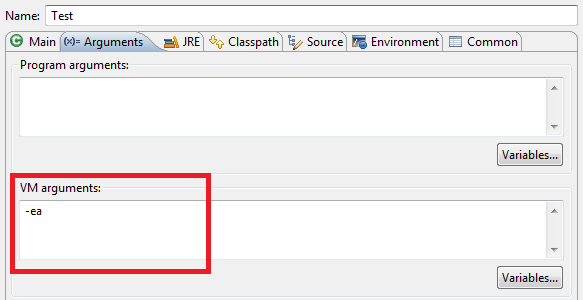
\includegraphics[width=0.8\columnwidth]{vmarg.png}%
  \end{figure}
  Alternativ: \hspace{1cm} \textit{java -ea MyClass}
\end{frame}

\section{JUnit}

\begin{frame}{Reminder}
\begin{block}{Übungsschein}
  \begin{itemize}
    \item Letztes Übungsblatt bis \textbf{03.02.2014} (20 Punkte + 10 Bonus)
    \item 60 Punkte $\rightarrow$ Übungsschein
  \end{itemize}
\end{block}
\pause
\begin{block}{Abschlussaufgaben}
  \begin{itemize}
    \item \textbf{Abschlussaufgabe 1} ab \textbf{17.2.14}
    \item \textbf{Abschlussaufgabe 2} ab \textbf{3.3.14}
    \item Bearbeitungszeit jeweils 4 Wochen
    \item Wird \textbf{nicht} von den Tutoren korrigiert!
   \end{itemize}
\end{block}
\end{frame}

\begin{frame}{Whats next?}
        \begin{figure}%
  
\includegraphics[width=0.4\columnwidth]{Man-question-mark.png}%
  \end{figure}
\end{frame}

\appendix
\beginbackup

%\begin{frame}[allowframebreaks]{References}
%        \printbibliography
%\end{frame}

\backupend

\end{document}